\chapter{Equity}
\label{chap:equity}

 One of the emerging challenges in \acrfull{CEd} refers to diversity \cite[p.~19:2]{burgstahler:2011}. Existing differences in a classroom can be a source of wealth and beauty. But they can also be a source of tensions that can generate conflicts. These conflicts are directly associated with the existence of privilege deriving from these differences.
 
According to \citeonline[p.~1]{parker:2015}, privilege is “an unearned, unasked-for advantage gained because of the way society views an aspect of a student’s identity, such as race, ethnicity, gender, socioeconomic status, and language”. The \gls{IBGE}\footnote{IBGE stands for \textit{Instituto Brasileiro de Geografia e Estatística} in Brazilian Portuguese.} conducted the \gls{PNAD Contínua}\footnote{PNAD Contínua stands for \textit{Pesquisa Nacional por Amostra de Domicílios Contínua} in Brazilian Portuguese.} in 2018, relating the theme of Information and Communication Technology. This survey revealed that one in four Brazilian people does not have internet access. Suppose we admit that a fraction of these Brazilians who do not have internet access were composed of students in an undergraduate computing program. What would be the impact of this reality on their education quality? What would be the difference in the education quality of these students relating to others? Scenarios like this show that the differences can convert in privilege to a specific social stratum of the scholar community.

The understanding that there is inequality in the conditions of student's context is fundamental for promoting social justice in \acrfull{CSE}. This perception allows the professor to reorganize their priorities and build a more honest frame of emerging problems deriving from the diversity of their scholar community.

Some concepts are essential when we refer to inequality of opportunities in education. \citeonline[p.~482]{lewis:2019} assert that:
\begin{citacao}
    “\textit{Equality} refers to the state where everyone has or is allocated the same things in the same degree, whereas \textit{equity} typically refers to having access to what is needed. [...] In general, [...] equity, and not equality, defines fair and just learning opportunities” (my emphasis).
\end{citacao}
An exciting way to understand the two concepts is by employing an illustration\footnote{Angus Maguire created this illustration and made it available in his portfolio: \url{http://madewithangus.com/portfolio/equality-vs-equity/.}} (Figure \ref{fig:equality-vs-equity}). The equality of conditions does not necessarily guarantee the real equality of opportunities. If we want everybody to have a real chance to watch the match, there must be a differentiated and intentional treatment. 

\begin{figure}[ht!]
\centering

\caption{\textmd{Illustration about the difference between equality and equity.}}
\label{fig:equality-vs-equity}
\fcolorbox{gray}{white}{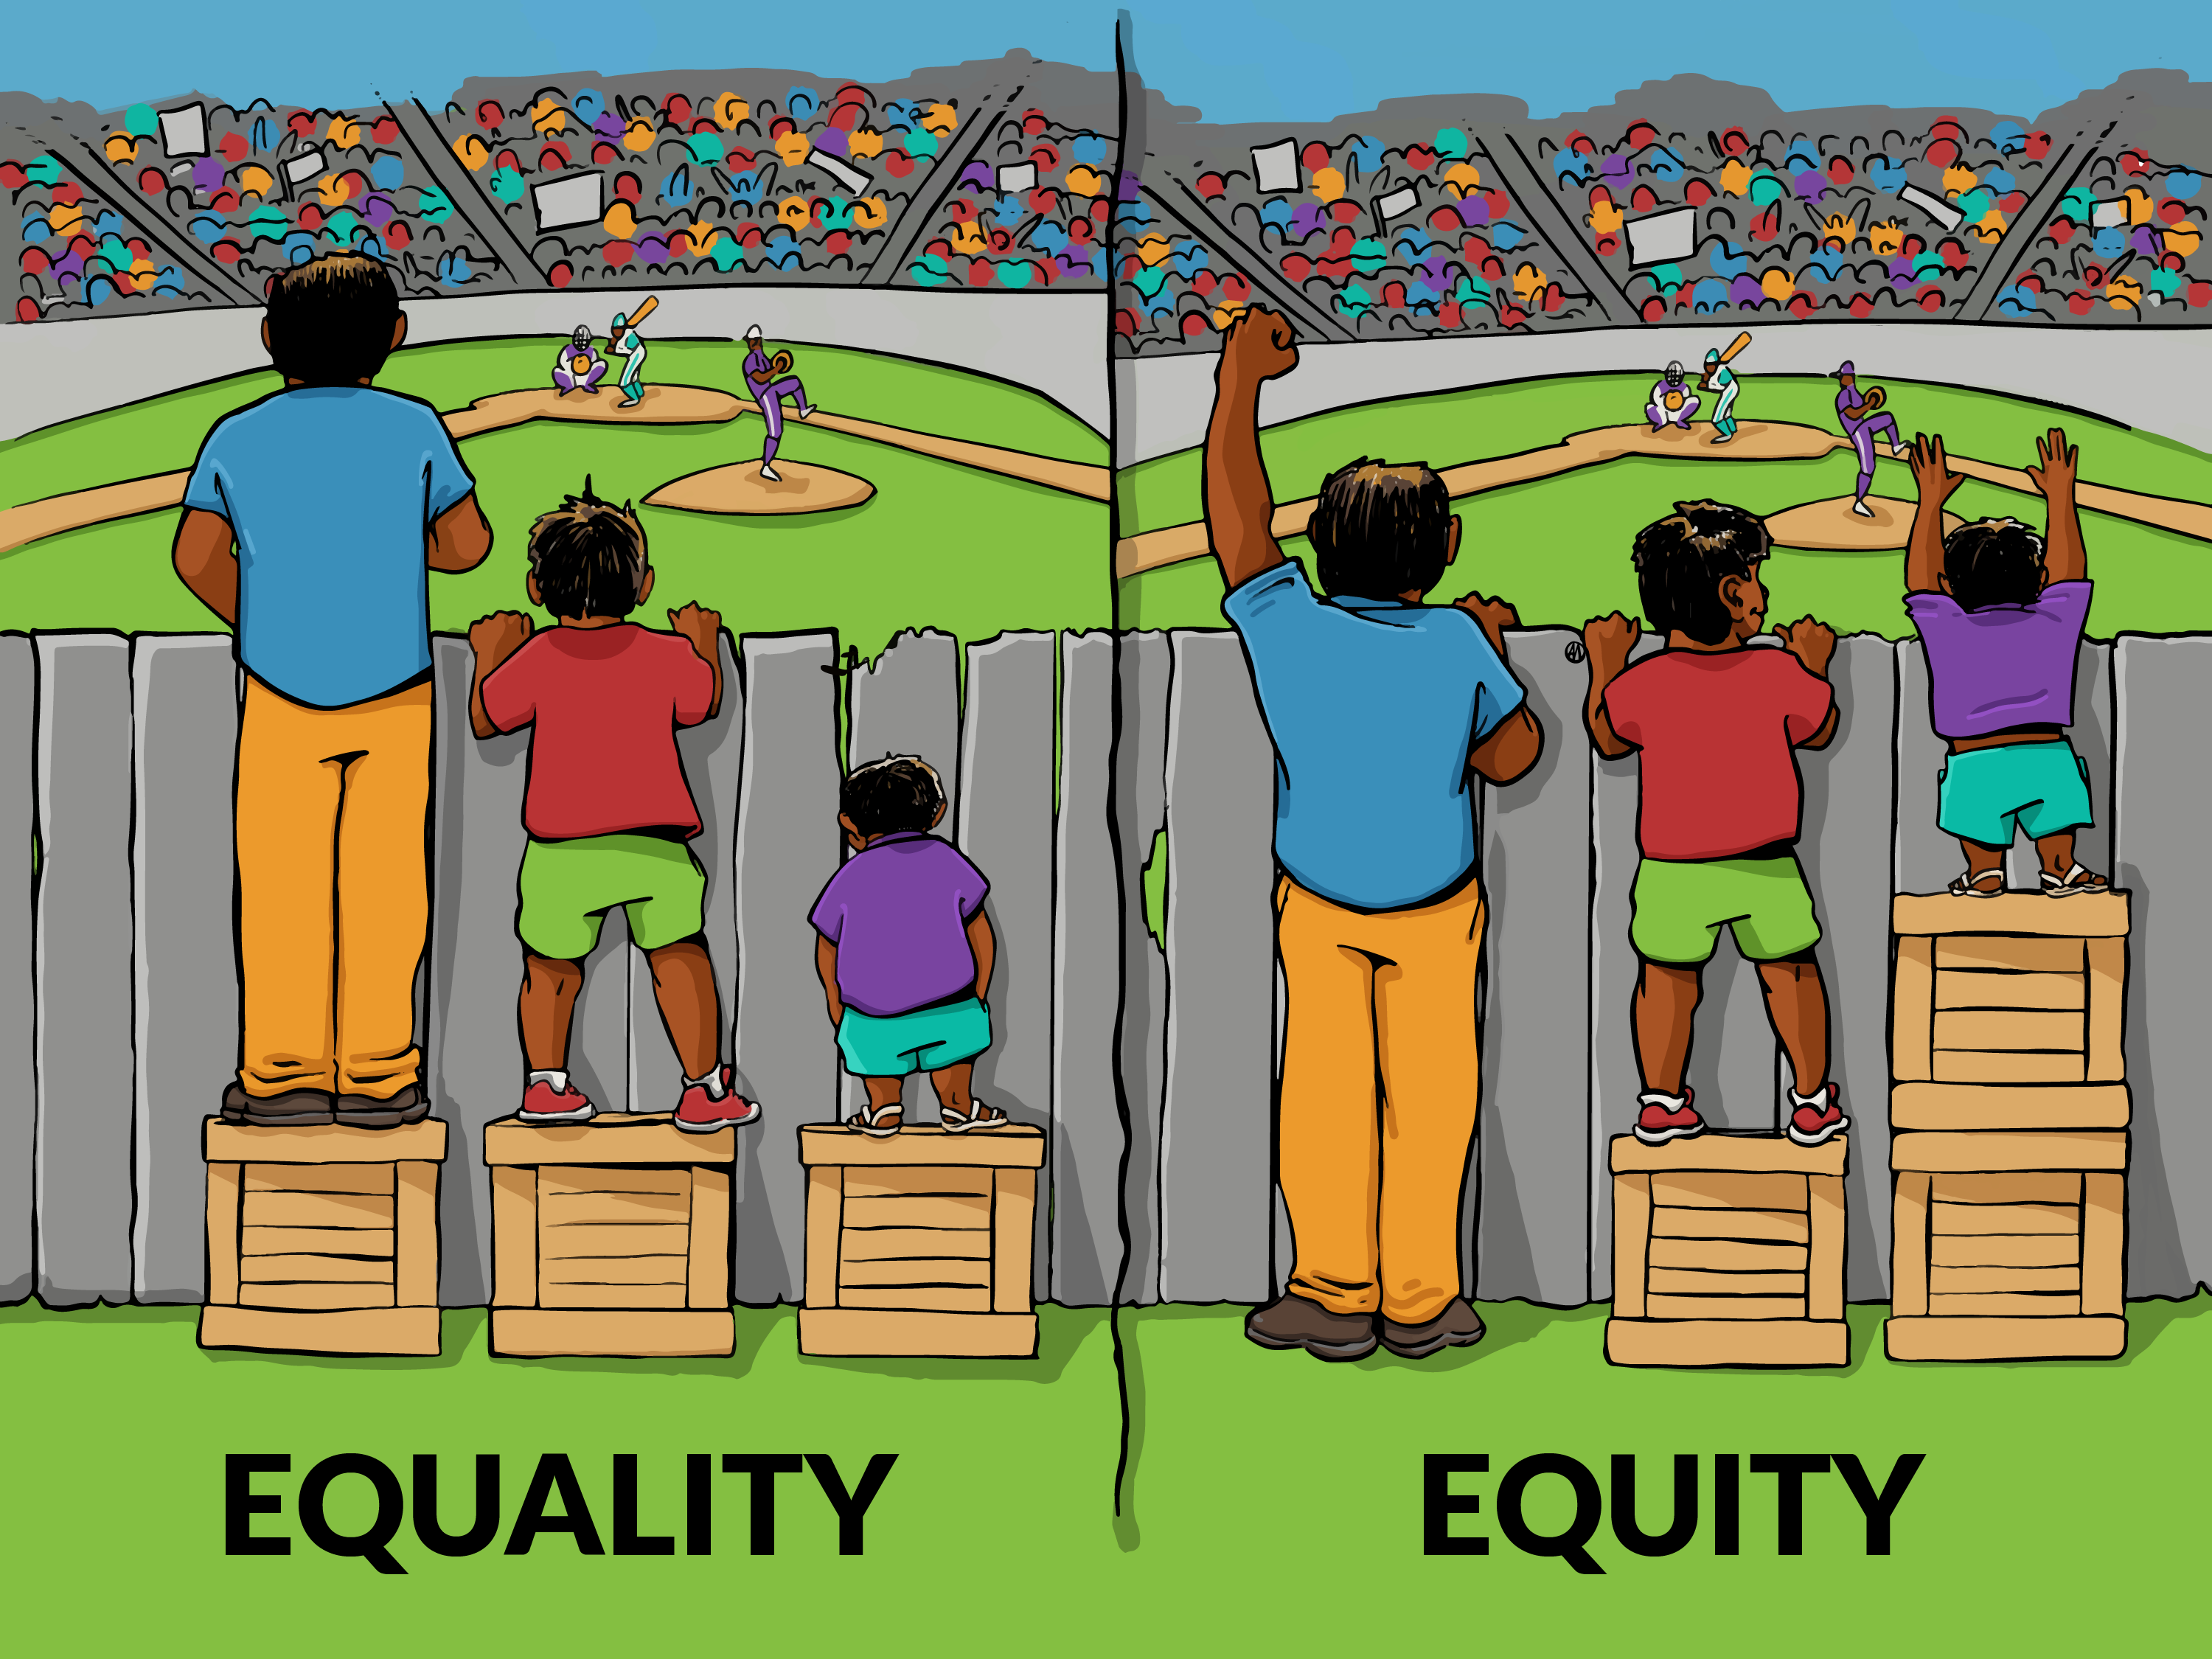
\includegraphics[width=0.7\textwidth]{images/chapter-03/equality-vs-equity.png}}

\par\medskip\ABNTEXfontereduzida\selectfont\textbf{Source:} Created by Angus Maguire \cite{maguire:2016}.%\citeauthor{manualufpe2020} (\citeyear{manualufpe2020}) \par\medskip
\end{figure}

Throughout this chapter, I detail the consequences of admitting this differentiated treatment to promote social justice in \gls{CSE}. Section \ref{equity-sec:diff-prin} shows the difference principle proposed by John Rawls. Section \ref{equity-sec:sen-ca} explains the capability approach of Amartya Sen and what it advances in the discussion about equity. Section \ref{equity-sec:cape} details the \gls{CAPE} framework, eliciting its elements, and how it has been used to analyze \gls{CSE} equity issues. Section \ref{equity-sec:br-context} describes the Brazilian context concerning the adoption of affirmative actions in higher education. And, at last, Section \ref{equity-sec:active-learning} points out the emergent issues when we investigate equity in active methodologies in \gls{CEd}.
